\section{System R}

System R ist ein von IBM in den 1970er Jahren durchgeführtes Datenbank Research Projekt \cite{selinger1979access}, \cite{wade2012ibm}, \cite{chamberlin1981history}, \cite{astrahan1976system}, \cite{astrahan1978system}. Es gilt insbesondere auf Grund von zwei Aspekten als der Pinoneer für moderne Datenbanksysteme: Auf der einen Seite wurde in System R zum ersten Mal \ac{SQL} implementiert. Auf der anderen Seite war es das erste System, das die Leistungsfähigkeit von relationalen Datenbanksystemen unter Beweis stellte. Fundamentale Design Entscheidungen, wie dynamische Programmierungsalgorithmen für \ac{QO}, prägen die weitere Entwicklung von Datenbanksystemen. System R gilt als der Vorgänger von IBMs DB2 und als Grundlage für viele andere Datenbanksysteme.


\subsection{Architektur und Systemstruktur}

\begin{figure}[h]
  \centering
  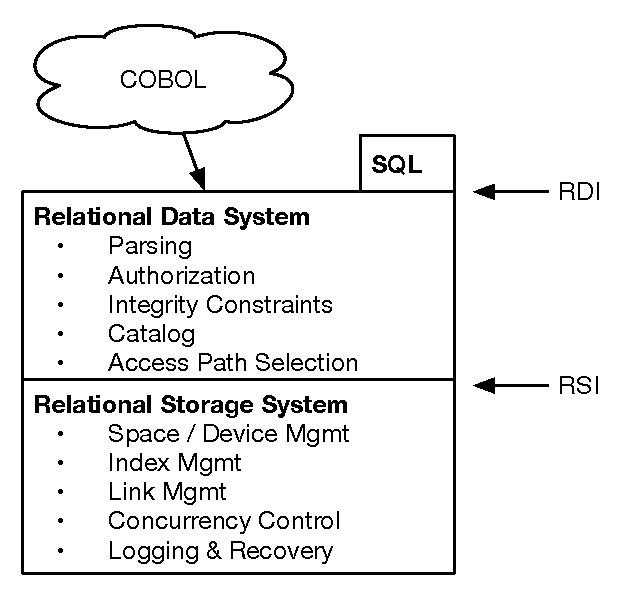
\includegraphics{03_Related_Work/SystemR.pdf}
  \caption{System R Architektur \cite{astrahan1976system} \cite{astrahan1978system}}
  \label{SystemRArchitecture}
\end{figure}


Wie in Abbildung \ref{SystemRArchitecture} zu erkennen,  besteht das System aus zwei Teilsystemen: \ac{RSS}, das dem RTS entspricht, und \ac{RDS}, das äquivalent zu einem CTS ist.

Das \ac{RSS} ist für die physische Verwaltung der Datenbank verantwortlich. Es kontrolliert u.a. die Speicherverwaltung, das Device-Management, die Transaktionskonsistenz und die Transations- sowie System-Wiederherstellung. Im Besonderen fällt in den Aufgabenbereich den Zugriff auf einzelne Tupel von Base Relations. Diese Funktionen werden gegenüber des \ac{RDS} mit Hilfe des \ac{RSI} bereitgestellt.

Das \ac{RDS} übernimmt via \ac{RDI} die Kommunikation nach Außen und leitet Befehle über das \ac{RSI} weiter. Anfragen von Außen werden mit Hilfe von \ac{SQL} an das System gestellt. Es ist auch möglich, dass externe Sprachen wie Cobol verwendet werden, die ohne Weiteres mit dem \ac{RDI} kommunizieren. In diesen Fällen muss SQL nicht verwendet werden. Das \ac{RSS} wandelt die Umfrage in eine für das \ac{RSI} verständliche Form um. Über das RSI wird die Anfrage entgegen genommen und ausgeführt.

<<<<<<< HEAD
=======
Das \ac{RDS} übernimmt mit Hife des \ac{RDI} die Kommunikation nach Außen und leitet Befehle über das \ac{RSI} weiter. Anfragen von Außen werden mit Hilfe von \ac{SQL} an das System gestellt. Es ist auch möglich, dass externe Sprachen wie beispielsweise Cobol verwendet werden, die ohne Weiteres mit dem \ac{RDI} kommunizieren. In diesen Fällen muss SQL nicht verwendet werden. Das \ac{RSS} wandelt die Umfrage in eine für das \ac{RSI} verständliche Form um. Über das RSI wird die Anfrage entegen genommen und ausgeführt.

>>>>>>> 2dbe3382d95b975a93a2c2789dd91dda3468d5cc



\subsection{Verarbeitung von Anfragen}

Wie bei anderen relationalen Datenbanksystemen steht am Beginn eine in \ac{SQL} formulierte Anfrage. Diese Anfrage wird in vier Schritten verarbeitet: Parsen,  Optimieren, Code Generierung und Ausführen.

Im ersten Schritt, Parsen, wird wie bei späteren Systemen die Syntax geprüft und die Anfrage in eine interne Repräsentation umgewandelt. Bei System R werden hierzu Query Blöcke verwendet. Sie repräsentieren die Anfrage mit einer SELECT list, einer FROM list und einem WHERE Baum. Er beinhaltet eine Liste der Elemente, die beispielsweise zum JOIN von Tabellen und der Einschränkung von Datensätzen dienen. Es ist möglich, dass mehrere Query Blöcke für eine einzige Anfrage vorhanden sind. Dies geschieht dann, wenn eine Anfrage Inner-Queries verwendet bzw. Anfragen als Argumente für eine WHERE Bedingung zum Einsatz kommen.


Sobald die Anfrage in Query Blöcke verarbeitet wurde, kommt der \ac{QO} zum Einsatz. Der Optimierer prüft zuerst, ob die genutzten Relationen und Felder auch in der Datenbank vorhanden sind und schlägt Informationen über diese im System R Catalog nach. Teil dieser Informationen sind statistische Informationen der referenzierten Relationen. Diese werden später für die Auswahl der richtigen Access Plans verwendet.

Im nächsten Schritt, optimieren, bestimmt der Optimizer für jeden Query Block den optimalen Access-Pfad. Zuerst wird die Evaluationsreihenfolge der Query Blocks im Statement festgelegt. Dann wird für jeden Query Block die FROM Relationen betrachtet. Sind mehr als eine Relation vorhanden, werden Permutationen der JOIN-Order gebildet. Es wird der Pfad mit den günstigsten Kosten gewählt und die notwendigen Modifikationen werden an der Anfrage vorgenommen. Das Resultat des Prozesses ist ein Plan in der \ac{ASL}.

Nachdem der Plan gefunden und als \ac{ASL}-Tree vorhanden ist, kommt der Code Generator zum Einsatz. Er übersetzt den \ac{ASL}-Plan in einen  Maschinencode. Dieser Code führt die Anfrage des Nutzers auf der Datenbank aus. 

Der Maschinencode wird dann auf dem \ac{RSS} über das \ac{RSI} ausgeführt und das Ergebnis zurückgegeben.

\subsection{Kostenberechnung}
Bei der Auswahl des optimalen Plans beginnt System R mit der Reihenfolge der Query Blocks. Zuerst wird für jeden Query Block geprüft, ob mehrere Tabellen in den FROM Listen vorhanden sind. Falls das der Fall ist, wird die Optimale Join-Order und die Methode des Joins bestimmt. Der Plan mit den geringsten Gesamtkosten für einen Block wird ausgewählt.

Zur Bestimmung der Kosten werden statistische Informationen aus dem System R Catalog herangezogen. Die Berechnung der Kosten für einen Access Plan, werden mit Hilfe der folgenden Funktion abgeschätzt:

$$Cost = Page Fetches + W * (RSI calls)$$


$Page Fetches$ repräsentieren die I/O Operationen, die beispielsweise durch den Abruf der Index Pages und der eigentlichen Pages entsteht. $RSI calls$ ist die Anzahl der erwarteten Datensätze, die durch das \ac{RSS} zurückgegeben werden. Sie dient als Abschätzung wie hoch der CPU Aufwand für die Rückgabe der Werte ist. Mit Hilfe des Parameters $W$ wird eingestellt in welchem Verhältnis I/O zu CPU Kosten stehen.


<<<<<<< HEAD
%\sout{Bei der Auswahl eines Plans unterscheidet das System zwischen einer \"interessanten\" Reihenfolge, also sortierten Ergebnissen, und einer ungeordneten Reihenfolge. Als interessante Reihenfolge, werden Reihenfolgen betrachtet, die gesamter Reihenfolge notwendig sind und die Kosten, die für das lesen in ungeordneter Reihenfolge notwendig sind und addiert auf diese Kosten, die Kosten für das Ordnen der Ergebnisse falls eine ungeordnete Reihenfolge + das Ordnen der Ergebnisse gemeinsam kürzer dauert als das direkte Ausgeben einer interessanten Reihenfolge wird sich für die günstigere Variante entschieden.}


Die Berechnung findet auf Basis der Daten statt, die von System Rs Catalog bereitgestellt werden. Die Daten umfassen folgende Kennzahlen:

\begin{itemize}
\item $R$: Kardinalität der Relation (Anzahl Tupel)
\item $D$: Anzahl der Daten-Pages, die von der Relation belegt werden
\item $T$: Durchschnittliche Anzahl der Tupel pro Daten Page (gleich $G/D$).
\item $H$: Koeffizient der CPU-Kosten ($1/H$ ist die Anzahl der Tupelvergleiche, die  als gleich den Kosten für einen Page Access sind.)
\end{itemize}

Auf Basis dieser Kennzahlen wird je nach Operator die Kosten festgestellt. 

%\sout{Die Berechnung geschieht auf Daten, die durch den Catalog bereitgestellt werden, Sie enthalten Informationen über die Kardinalität und die Anzahl der Segmente, die für das auslesen einer Relation notwendig sind, ebenfalls wird ein Selektivitätsfaktor genutzt, der das Verhältnis der Gesamtheit zur eingeschlossenen Menge der Anfrage angibt. Sprich die Menge der ausgeschlossenen Tupel.}


=======
Bei der Auswahl eines Plans unterscheidet das System zwischen einer "interessanten" Reihenfolge, also sortierten Ergebnissen, und einer ungeordneten Reihenfolge. Als interessante Reihenfolge, werden Reihenfolgen betrachtet, die gesamter Reihenfolge“ notwendig sind und die Kosten, die für das lesen in ungeordneter Reihenfolge notwendig sind und addiert auf diese Kosten, die Kosten für das Ordnen der Ergebnisse falls eine ungeordnete Reihenfolge + das Ordnen der Ergebnisse gemeinsam kürzer dauert als das direkte Ausgeben einer interessanten Reihenfolge wird sich für die günstigere Variante entschieden. 

Die Berechnung geschieht auf Daten, die durch den Catalog bereitgestellt werden, Sie enthalten Informationen über die Kardinalität und die Anzahl der Segmente, die für das auslesen einer Relation notwendig sind, ebenfalls wird ein Selektivitätsfaktor genutzt, der das Verhältnis der Gesamtheit zur eingeschlossenen Menge der Anfrage angibt. Sprich die Menge der ausgeschlossenen Tupel.
>>>>>>> 2dbe3382d95b975a93a2c2789dd91dda3468d5cc

\subsection{Plan Enumerator}
Die Enumeration des System R Optimizers zeigt zwei wichtige Aspekte eines Enumerators: Auf der einen Seite die \"interesting Order\" auf der anderen Seite \"dynamic programming\". 

Dynamische Programmierung geht davon aus, dass das Kostenmodell dem Optimalitätsprinzip von Bellman \cite{Bellman:1957} gehorcht. Das Prinzip sagt aus, dass sich eine Optimallösung aus optimalen Teillösungen zusammensetzt. In unserem konkreten Fall sagt das Prinzip das der optimale Plan nur aus optimalen Teilbäumen bestehen kann. Somit müssen nur optimale Subplans zur Erzeugung des optimalen Plans verwendet werden. i.a.w. Sucht man mit Hilfe eine bottom-up Enumeration Algorithmus nach dem optimalen Plan. So müssen nur Subpläne in Betracht für eine optimale gesamt Lösung gezogen werden, die für sich optimal sind. 

Ein weiterer wichtiger Aspekt von System R ist die Verwendung von Intersting Orders. Als Interesting Orders werden Reihenfolgen, die innerhalb eines Joins entstehen bezeichnet, die zwar höhere direkte Kosten verursachen, jedoch zu niedrigeren Gesamtkosten beitragen können. So ist es möglich, dass die Kosten durch einen Nested-Loop Join zwar höher sind als durch einen Merge-Join, allerdings die Gesamtkostenbilanz durch den teureren Nested-Loop Join positiv beeinflusst wird. Gerade beim Einsatz von Prunning Algorithmen ist es möglich, dass so ein global subpotimaler Plan gewählt wird. System R identifiziert diese geordneten Resultate, die für die zukünftige Ausführung von Vorteil sein können. Außerdem werden Pläne in System R nur dann verglichen, wenn sie die selbe Reihenfolge und den selben Ausdruck besitzen. 